\documentclass{standalone}
\usepackage{graphicx}	
\usepackage{amssymb, amsmath, amsthm}
\usepackage{color}

\usepackage{tikz}
\usetikzlibrary{intersections, backgrounds}
\definecolor{light}{RGB}{179, 255, 255}
\definecolor{light_highlight}{RGB}{154, 246,255}
\definecolor{mid}{RGB}{103,195,255}
\definecolor{mid_highlight}{RGB}{52,144,204}
\definecolor{dark}{RGB}{1,93,153}
\definecolor{dark_highlight}{RGB}{0,42,102}
\definecolor{gray10}{gray}{0.1}
\definecolor{gray20}{gray}{0.2}
\definecolor{gray30}{gray}{0.3}
\definecolor{gray40}{gray}{0.4}
\definecolor{gray60}{gray}{0.6}
\definecolor{gray70}{gray}{0.7}
\definecolor{gray80}{gray}{0.8}
\definecolor{gray90}{gray}{0.9}
\definecolor{gray95}{gray}{0.95}


\begin{document}

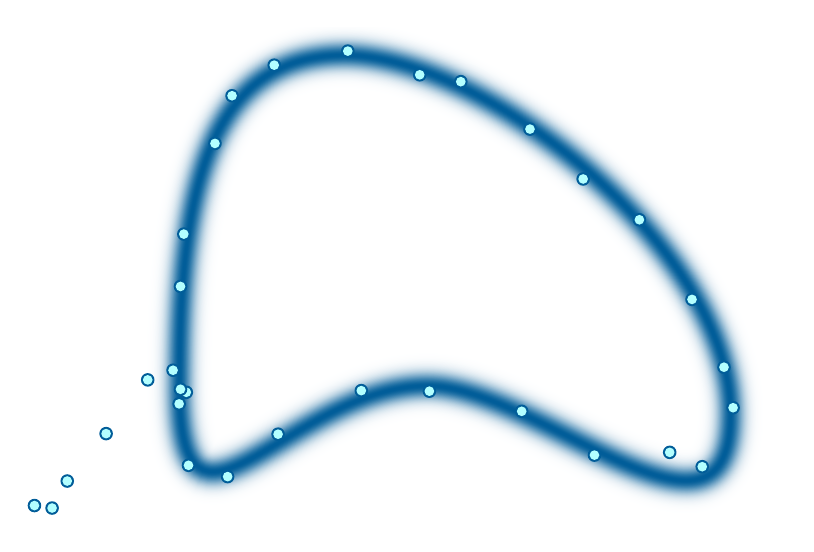
\begin{tikzpicture}[scale=0.35, thick]

    \begin{scope}
        \clip (-12, -7) rectangle (12, 11);
        \foreach \i in {1, 0.99, ..., 0} {
                \pgfmathsetmacro{\prop}{100 * exp(-10.0 * \i * \i)};
                \colorlet{custom}{dark!\prop!white};
                \draw[line width={30
                            * \i}, color=custom]
                (-10, -2) .. controls (-10, 5) and (-9, 10) .. (-4, 10)
                .. controls (1, 10) and (10, 3) .. (10, -3)
                .. controls (10, -9) and (3, -2) .. (-1, -2)
                .. controls (-6, -2) and (-10, -9) .. (-10, -2);
            }

    \end{scope}
    \fill[color=dark] (-15.26, -6.34) circle (7pt);
\fill[color=light] (-15.26, -6.34) circle (5pt);
\fill[color=dark] (-14.62, -6.43) circle (7pt);
\fill[color=light] (-14.62, -6.43) circle (5pt);
\fill[color=dark] (-14.07, -5.45) circle (7pt);
\fill[color=light] (-14.07, -5.45) circle (5pt);
\fill[color=dark] (-12.66, -3.73) circle (7pt);
\fill[color=light] (-12.66, -3.73) circle (5pt);
\fill[color=dark] (-11.15, -1.78) circle (7pt);
\fill[color=light] (-11.15, -1.78) circle (5pt);
\fill[color=dark] (-10.23, -1.43) circle (7pt);
\fill[color=light] (-10.23, -1.43) circle (5pt);
\fill[color=dark] (-10.01, -2.65) circle (7pt);
\fill[color=light] (-10.01, -2.65) circle (5pt);

    \fill[color=dark] (-9.75, -2.23) circle (7pt);
\fill[color=light] (-9.75, -2.23) circle (5pt);
\fill[color=dark] (-9.96, 1.61) circle (7pt);
\fill[color=light] (-9.96, 1.61) circle (5pt);
\fill[color=dark] (-9.84, 3.51) circle (7pt);
\fill[color=light] (-9.84, 3.51) circle (5pt);
\fill[color=dark] (-8.71, 6.80) circle (7pt);
\fill[color=light] (-8.71, 6.80) circle (5pt);
\fill[color=dark] (-8.09, 8.53) circle (7pt);
\fill[color=light] (-8.09, 8.53) circle (5pt);
\fill[color=dark] (-6.56, 9.64) circle (7pt);
\fill[color=light] (-6.56, 9.64) circle (5pt);
\fill[color=dark] (-3.89, 10.15) circle (7pt);
\fill[color=light] (-3.89, 10.15) circle (5pt);
\fill[color=dark] (-1.28, 9.29) circle (7pt);
\fill[color=light] (-1.28, 9.29) circle (5pt);
\fill[color=dark] (0.21, 9.04) circle (7pt);
\fill[color=light] (0.21, 9.04) circle (5pt);
\fill[color=dark] (2.72, 7.32) circle (7pt);
\fill[color=light] (2.72, 7.32) circle (5pt);
\fill[color=dark] (4.65, 5.51) circle (7pt);
\fill[color=light] (4.65, 5.51) circle (5pt);
\fill[color=dark] (6.69, 4.03) circle (7pt);
\fill[color=light] (6.69, 4.03) circle (5pt);
\fill[color=dark] (8.60, 1.14) circle (7pt);
\fill[color=light] (8.60, 1.14) circle (5pt);
\fill[color=dark] (9.76, -1.32) circle (7pt);
\fill[color=light] (9.76, -1.32) circle (5pt);
\fill[color=dark] (10.09, -2.79) circle (7pt);
\fill[color=light] (10.09, -2.79) circle (5pt);
\fill[color=dark] (8.97, -4.93) circle (7pt);
\fill[color=light] (8.97, -4.93) circle (5pt);
\fill[color=dark] (7.79, -4.41) circle (7pt);
\fill[color=light] (7.79, -4.41) circle (5pt);
\fill[color=dark] (5.06, -4.51) circle (7pt);
\fill[color=light] (5.06, -4.51) circle (5pt);
\fill[color=dark] (2.42, -2.92) circle (7pt);
\fill[color=light] (2.42, -2.92) circle (5pt);
\fill[color=dark] (-0.93, -2.19) circle (7pt);
\fill[color=light] (-0.93, -2.19) circle (5pt);
\fill[color=dark] (-3.40, -2.17) circle (7pt);
\fill[color=light] (-3.40, -2.17) circle (5pt);
\fill[color=dark] (-6.42, -3.75) circle (7pt);
\fill[color=light] (-6.42, -3.75) circle (5pt);
\fill[color=dark] (-8.25, -5.29) circle (7pt);
\fill[color=light] (-8.25, -5.29) circle (5pt);
\fill[color=dark] (-9.67, -4.88) circle (7pt);
\fill[color=light] (-9.67, -4.88) circle (5pt);
\fill[color=dark] (-9.96, -2.12) circle (7pt);
\fill[color=light] (-9.96, -2.12) circle (5pt);



\end{tikzpicture}



\end{document}